\chapter{Modelling a Database for Dynamic Multimedia Data}
\label{chapter:system_model}

We have elaborated in \Cref{chapter:applications}, multimedia retrieval and analytics workloads (and workloads that exhibit similiar characteristics) pose specific requirements on any data management system. In this chapter, focus on the following four aspects and derive a formal model to accomodate them on a system level:

\begin{description}
    \item[Support for Non-atomic Data] Multimedia workloads process features, which are usually real-valued, high-dimensional vectors but can theoretically be any mathematical object (e.g., complex numbers, matrices etc.). A multimedia \acrshort{dbms} must support these objects as first-class citizens.
    \item[Support for Distance Computation] The notion of proximity between features plays a crucial role in all types of multimedia workloads, be it for simple \acrshort{nns} or clustering. While certain workloads rely on raw speed for simple computations and data structures that allow for this type of lookup, other workloads require the ability to compose more complex computations and execute them efficiently without the use of an index. Both aspects must be covered by a multimedia \acrshort{dbms}.
    \item[Dynamically Changing Data] Data is usually subject to constant change and a multimedia \acrshort{dbms} must be able to propagate these changes to all the relevant data structures while maintaining ther internal consistency model.
    \item[Accuracy vs. Time] Multimedia queries often trade retrieval accuracy against speed or vice-versa, e.g., when using a high-dimensional indexes. The multimedia \acrshort{dbms} must allow the user to express their perference at different levels of the system.
\end{description}

To address these requirements, we propose and formalize a set of functionality, which will be specified in the next sections. First, we propose a notion of \emph{generalized, proximity based queries} as an extension to the relational model. Second, we describe a \emph{cost-model} that takes the notion of accuracy of results into acount. And finally, we introduce a general-purpose mechanism to enable high-dimensional indexes to cope with changing data.

All these contributions can be seen as extensions to the functionality provided by a traditional \acrshort{dbms}. For the sake of argument we assume, without loss of generality, we assume the relational model and \acrshort{acid} properties for the model \acrshort{dbms} under consideration.

\section{Generalized Proximity Based Operations}

Starting with the vector space model for similarity search~\cite{Zezula:2006Similarity} presented in \Cref{chapter:theory_multimedia_analysis_and_retrieval}, we propose to extend the notion of distance-based similarity search to that of a more general \emph{proximity based query} following \cref{definition:pbq}.

\begin{definition}[label=definition:pbq]{Proximity Based Query}{}
    Let $\relation$ be a relation. Any database query that relies on the evaluation of a distance function $\delta: \domain_{f} \times \domain_{f} \rightarrow \mathbb{R}_{\geq 0}$ that calculates the distance between an attribute $\attribute_{p} \in \schema(\relation)$ and some query $q \in \domain_f$, is called a \emph{proximity based query}. We call $q$ the \emph{query} and $\attribute_{p}$ the \emph{probing argument}, which both share the same \emph{query data domain} $\domain_f$. It is to be noted, that $\domain_f \equiv \symfeatures$. 
\end{definition}

\cref{definition:pbq} simply requires a notion of proximity between some attribute and a query to be obtained by evaluating some distance function. The definition does not make any assumption as to what data domains $\domain_f$ query and probing attribute belong to nor how the distance is being used within the query. 

It is obvious, that similarity search falls into the broader category of a proximity based query, wherein the distance is used to rank a relation and subsequently limit its cardinality. In addition to this common application, the definition of proximity based queries also includes operations such as evaluating a distance function followed by some filtering (e.g., range search) or aggregation based on the computed value (e.g., clustering). That is, we are not limited to mere \acrshort{nns}, since we consider obtaining the distance as one step, which can be freely combined with all other operations supported by the underlying algebra.

\subsection{Revisiting Distance Computation}

Since the choice of the distance function $\symdist$ is a crucial part of any proximity based query, it is worth revisiting its definition. Again, starting with the metric space modell~\cite{Zezula:2006Similarity}, we identify the following (implicit) constraints with respect to the distance function:

\begin{enumerate}
    \item The domain (i.e., the input) of the distance function $\symdist$ is assumed to be $\mathbb{R}^{dim} \times \mathbb{R}^{dim}$, that is, the distance function is assumed to be a binary function and arguments are restricted to real-valued vectors.
    \item The codomain (i.e., the output) of the distance function $\symdist$ is assumed to be $\mathbb{R}_{\geq 0}$, hence, the generated distance value is a positive, real number.
    \item The pair $(\domain_f,\symdist)$ usually constitutes a metric, thus satisfying the non-negativity, identity of indiscernibles, symmetry and subadditivity properties.
\end{enumerate}

Upon closer examination and if we consider the use cases presented in \Cref{chapter:applications}, one must come to challenge some of these constraints. If, for example, we turn to \cref{example:mrf}, we realise that it is not reasonable to impose a general restriction of the domain of the distance function to $\mathbb{R}^{dim}$ with $dim \in \mathbb{N^{+}}$

\begin{example}[label=example:mrf]{\acrlong{mips}{} for \acrshort{mrf}}{}
    In \acrshort{mrf} (see \cref{section:application_mrf}), we try to obtain the signal vector $a_{i \in \mathbb{N}} \in \domain_f \subset \mathbb{C}^{dim}$ so that it maximizes the inner product to a signal (query) vector $q \in \mathbb{C}^{dim}$. In this case, the distance function $\symdist$ has the form $\symdist \colon \mathbb{C}^{dim} \times \mathbb{C}^{dim} \to \mathbb{R}_{\geq 0}$. Hence, the domain of $\symdist$ is a complex vector space.
\end{example}

Obviously, this limitation of the definition of $\symdist$ can be easily remediated simply by extending the set of supported data domains $\domainset$ by $\mathbb{C}^{dim}$ similarily to how it was done for $\mathbb{R}^{dim}$ as proposed by \cite{Giangreco:2018Database}. Nevertheless, we have to acknowledge, that the text-book definition of a distance function is obviously too limited for some real-world applications, and that the query and probing arguments of a distance function could be any type of value supported by the \acrshort{dbms}. Another, similar example could be the \emph{Levenshtein distance}~\cite{Levensthtein:1965Binary} -- often used in computer linguistics -- which is a distance metric on string values.

If now in addition, we consider \cref{example:svmdistance}, we see that restricting oneself to binary functions with $\mathbb{R}_{\geq 0}$ is also too limiting when facing certain practical scenarios.

\begin{example}[label=example:svmdistance]{Distance Between a Vector and a Hyperplane}{}
    To find positive and negative examples $a_{i} \in \domain_f \subset \mathbb{R}^{dim}$ given a linear classifier, e.g., provided by a SVM, we evaluate the distances between the attributes and a (query-)hyperplane described as $\mathbf{q}^T\mathbf{x} - b = 0$ with $\mathbf{q},\mathbf{x} \in \mathbb{R}^{dim}$ and $b \in \mathbb{R}$. The distance function is then given by:

    \begin{equation}
        \symdist (\mathbf{a}_i, \mathbf{q}, b) = \frac{\left\|\mathbf{q}^T \mathbf{a_i} + b \right\|}{\left\|\mathbf{q}\right\|}
    \end{equation}
    
    $\symdist$ now has the form $\symdist \colon \mathbb{R}^{dim} \times \mathbb{R}^{dim} \times \mathbb{R} \to \mathbb{R}$. Hence, $\delta$ is no longer a binary but a ternay function with arguments $\mathbf{a_{i}}$, $\mathbf{q}$ and $b$. Furthermore, the distance may take negative values depending on whether a result is considered a positive or negative example.
\end{example}


Again, we are confronted with an example that violates the text-book definition of a distance function. While the idealized idea that distance functions used in proximity based queries must always constitute a metric on some real-valued vector space may be very common~\cite{Zezula:2006Similarity}, we see in practice that this assumption is often violated~\cite{Skopal:2011Nonmetric,Bernhauer:2019Nonmetric} and that many functions used to calculate proximity between objects, are not actual metrics. Even though, this can be a disadvantage when considering high-dimensional index structures that exploit the geometric properties of metric spaces, it is obvious that such functions exist and must thus be considered in any generalized database application supporting proximity based queries. 

In contrast, there is actually good reason to assume the codomain of a distance function  $\symdist$ to lie in $\mathbb{R}$. On the one hand, it is obviously convenient both for the underlying mathematics as well as from an implementation prespective. More importantly, however, real numbers -- unlike, for example, complex numbers or vectors -- come with a natural, total ordering, which is required for downstream operations such as sorting, ranking or clustering.

To summarize, we have established that, on the one hand, we require a proper definition of what is considered to be a valid distance function so as to be able to efficiently plan and execute queries that use them, while on the other hand we must keep that definition open enough to accomodate the many different, applications.

To address the aforementioned limitations while still accomodating classical, metric distances, we propose the extension of a the distance function to the more general notion of a \acrfull{dfc} following \cref{definition:dfc}.

\begin{definition}[label=definition:dfc]{\acrlong{dfc}}{}
    A \acrshort{dfc} $\symdfc \colon \domain_f \times \domain_f \times \domain_{1} \ldots \times \domain_{N} \to \mathbb{R}$ is an N-ary but at least binary function $\symdfc(p,q,s_1,\ldots,s_n)$ that outputs a distance $d \in \mathbb{R}$ between a probing argument $p \in \domain_q$ and a query argument $q \in \domain_q$ using a defined number of \emph{support arguments} $s_{k \in \mathbb{N}}$ from any of the data domains in $\domainset$.

    As a convention for notation, the probing argument $p$ of a DFC $\symdfc(p,q,s_1,...,s_n)$ will always come first, followed by the query argument $q$, again followed by its support arguments $s_k$ in no particular order.
\end{definition}

\begin{example}[label=example:dfc]{Examples of \acrlong{dfc}es}{}

    A merely illustrative yet widely used example of a \acrshort{dfc} would be the family of \emph{Minkowski Distances} $\symdfc_{M} \colon \mathbb{R}^{dim} \times \mathbb{R}^{dim} \times \mathbb{R} \to \mathbb{R}_{\geq 0}$. In this context, support argument $m$ is used to convert the higher-order function to a classical distance function, such as, the Manhattan ($L_1$) or Euclidean ($L_2$) distance:

    \begin{equation}
        \symdfc_{M}(\mathbf{p},\mathbf{q},m) = \left(\sum_{i=1}^{n} \mid p_i - q_i \mid^m\right)^{\frac{1}{m}}
    \end{equation}
    
    \begin{equation}
       \symdist_{L1}(\mathbf{p},\mathbf{q}) = \texttt{IMP}_{m=1}(\symdfc_M) = \sum_{i=1}^{n} \mid p_i - q_i \mid
    \end{equation}
    
    \begin{equation}
       \symdist_{L2}(\mathbf{p},\mathbf{q}) = \texttt{IMP}_{m=2}(\symdfc_M) = \sqrt{\sum_{i=1}^{n} \mid p_i - q_i \mid^2}
    \end{equation}
    
    However, using the idea of a \acrshort{dfc}, we can express many different types of much more complex distance functions in a simple yet powerful framework. For example, the following distance function is used to obtain a dissimilarity between poses using the joint locations of an 18-keypoint skeleton (details presented in \cite{Heller:2022Multi}):

    \begin{equation}
        \hat{\delta}(\mathbf{p},\mathbf{q},\mathbf{w}_q,\mathbf{w}_f, s) = \sum_{i=1}^{n} \mid (p_i - q_i) \mid \min(w_{q,i}, w_{f,i}) + 2\pi (s - \sum_{i=1}^{n} \min(w_{q,i}, w_{f,i}))
    \end{equation}

    The query and support arguments $\mathbf{p}$ and $\mathbf{q}$ are the actual, normalised keypoints and are accompanied by two weight-vectors $\mathbf{w}_q$ and $\mathbf{w}_f$, that encode the presence or absence of a joint in a scene. To normalise for missing joints, a normalisation factor based on the weight-sum $s$ is employed.

\end{example}


A \acrshort{dfc} (and any function for that matter) is uniquely defined by its \emph{signature}, a ($N+1$)-tuple specifying the name of the \acrshort{dfc} and the data domains $\domain_i$ of the arguments it can accept as defined in \cref{equation:dfc_signature}.

\begin{equation}
    \label{equation:dfc_signature}
    \texttt{SIG}(\symdfc) = (\mathtt{NAME}, \domain_p, \domain_q, \domain_1,... \domain_{N-2})
\end{equation}

In the context a concrete execution plan for a proximity based query, we observe that most of the time, the query argument effectively remains constant, while the support arguments may or may not be subject to change. For example, for simple \acrshort{nns}, there is a single, constant query vector that is compared against all the vectors in the \acrshort{dbms}, i.e., the probing argument. Hence, irrespective of the arity of the \acrshort{dfc}, its (partial-) \emph{implementation} $\delta$ used during execution, comes with an arity of at most $N-1$. This is denoted by \cref{equation:dfc_implementation}.

\begin{equation}
    \label{equation:dfc_implementation}
    \symdist = \texttt{IMP}(\symdfc) \ni \texttt{SIG}(\symdist) \subset \texttt{SIG}(\symdfc)
\end{equation}

With this idea of a \acrshort{dfc} in mind, we can start to reason about their properties in the broader context of database operations in general and proximity based queries in particular:

\begin{description}
    \item[\acrshort{dfc} and Proximity Based Queries] In extension to \cref{definition:pbq}, we realise that any query execution plan that involves the evaluation of a (partial) implementation of a \acrshort{dfc}, falls into the category of a proximity based query.

    \item[Variable and Constant Arguments] In the context of a proximity based query, every attribute of a \acrshort{dfc} can either be regarded as \emph{constant} or variable. That is, as elements in the database are iterated during query execution, they either remain the same or assume new values. 
    
    \item[Purity of Domain] Since the purpose of a \acrshort{dfc} is to quantify proximity between a probing argument $p$ and a query argument $q$, we can assume that $p, q \in \domain_f$. Furthermore, we require that the query argument is always constant, wheras the probing argument is always variable.

    \item[Scalarity of Codomain] A \acrshort{dfc} and its implementations always produce a single, scalar output $d \in \symreal$ to quantify the distance.
\end{description}

All the aforementioned properties can be put to explicit use when planning for the execution of a query, be it for index selection, optimisaion of execution through caching as well as other measures.

As an aside, we must address the role of dimensionality $dim$ in the case of data domains that are subsets of vector spaces, i.e.,  $\domain_q \subset \mathbb{R}^{dim}$ or $\domain_q \subset \mathbb{C}^{dim}$. One could argue, that the dimensionality of such a vector space can also be seen as a parameter of the \acrshort{dfc}. Irrespective of the merits such an argument might have, we consider the dimensionality of the vector space to be a strictly structural property of the underlying data domain $\domain_q$ and thus a constant in the context of a query.

\subsection{Extending the Relational Model}

Using \cref{definition:dfc}, one can now start to integrate \acrshort{dfc}s into the relational data model. In line with~\cite{Giangreco:2018Database}, we first assume $\domainset$ -- the set system of data domains supported by the database -- to be extended by whatever data domain $\domain_q$ is required, such as but not limited to $\mathbb{R}^{dim}$ or $\mathbb{C}^{dim}$. 

\subsubsection{Extended Projection and DFCs}

We use the idea of an extended projection $\pi_{P}$ -- as proposed by \cite{Gupta:1995Generalized,Garcia:2009Database} and introduced in \cref{section:rel_extensions} -- wherein $P$ denotes a list of projection expressions $e$ that involve attributes $\attribute_i \in \relation$. That is, in addition to the simple projection onto attributes $\attribute_i$, an extended projection may also include the evaluation of literals or functions as expressed in \Cref{definition:extended_projection}. 

\begin{definition}[label=definition:extended_projection]{Extended Projection $\projection_P$}{}
Let $\relation$ be a N-ary relation over attributes $\attribute \in \schema (\relation)$ with tuples $t \in \relation$. We call $\projection_{P}$ the \emph{extended projection} with $K$ projection elements $e_i \in P$, i.e., $P = \{ p_1, p_2, \ldots p_K \}, \textrm{with} \: p_i \in \schema(\relation) \vee p_i \in \domain_{\mathcal{L}} \vee p_i \in \mathcal{F}$, where $\mathcal{F}$ denotes a set of all functions $f_i \colon \domain_{1} \times \domain_{2} \ldots \domain_{M} \rightarrow \domain_{out}$ known to the \acrshort{dbms} and $\domain_{\mathcal{L}} \in \domainset$ denotes the domain of literal values. The extended projection is then defined as follows:

\begin{equation*}
    \projection_{P}(\relation) =  \{ t\left[ P \right] : t \in \relation \} \textrm{ with } t\left[ P \right] = \bigcup_{p_i \in P }
    \begin{cases} 
        t \left[ p_i \right] & \text{if } p_i \in \schema(\relation) \\
        p_i  & \text{if } p_i \in \domain_{\mathcal{L}} \\
        p_i(t \left[ P^{'} \right]) & \text{if } p_i \in \mathcal{F} \\
    \end{cases}
\end{equation*}

Note, that the domain of every function $f_i \in \mathcal{F}$ is again, an implicit, extended projection $t \left[ P^{'}\right]$, where $P^{'}$ contains all projection elements required as function arguments. Hence, function invocations can be nested arbitrarily.

\end{definition}

If now we assume any DFC supported by the \acrshort{dbms} to be member of $\mathcal{F}$, the evaluation of a \acrshort{dfc} as part of a query is given by \Cref{definition:dfc_rel}. The application of both definitions \Cref{definition:extended_projection} and \Cref{definition:dfc_rel} is illustrated in \Cref{example:extended_projection_dfc}

\begin{definition}[label=definition:dfc_rel]{\acrlong{dfc} in Extended Projection $\pi_{P}$}{}
    Let $\symdfc \colon \domain_q \times \domain_q \times \domain_{1} \ldots \times \domain_{N-2} \to \mathbb{R}$ be a N-ary \acrshort{dfc}. The \emph{extended projection} $\pi_{\symdfc(p_1, p_2, \ldots p_N)}(\relation) \textrm { with } p_i \in \schema(\relation) \vee p_i \in \domain_{\mathcal{L}} \vee p_i \in \mathcal{F}$ denotes the evaluation of $\symdfc$ using $N$ arguments. Applying $\pi_{\symdfc(\cdot)}$ on a M-ary relation $\relation$ introduces a new distance attribute $\mathcal{A}_\delta$, i.e., $\mathtt{SCH}(\pi_{\symdfc(\cdot), \mathcal{A}_1, \ldots, \mathcal{A}_M}(\relation)) = \mathtt{SCH}(\relation) \cup \{ \mathcal{A}_{\symdfc} \}$
\end{definition}

\begin{example}[label=example:extended_projection_dfc]{Obtaining a Distance using Extended Projection}{}

    The following table lists the schema and extent of $\relation_{\mathtt{paintings}}$, which now contains a column of feature vectors in addition to the scalar attributes, i.e., $\domain_{\mathtt{feature}} \subset \symreal^3$.

    \begin{center}
        \begin{tabular}{ l || l | l | l | l |}
            $\relation_{\mathtt{painting}}$ & $\attributep_{\mathtt{title}}$  & $\attributef_{\mathtt{artist}}$ & $\attribute_{\mathtt{painted}}$ & $\attribute_{\mathtt{feature}}$ \\ 
            \hline
            \hline
            $t_1$ & Mona Lisa &  Leonardo da Vinci & 1506 &  $[2.0,7.0,-8.0]$ \\
            \hline
            $t_2$ & The Starry Night & Vincent van Gogh & 1889 & $[1.0,0.0,3.0]$ \\
            \hline
            $t_3$ & Las Meninas & Diego Velázquez & 1665 & $[-1.0,3.0,9.0]$ \\
            \hline
        \end{tabular}
    \end{center}

    The extended projection $\projection_{P} (\relation)$ with $P = (\attribute_{\mathtt{title}}, \symdist([0,0,0],\attribute_{\mathtt{feature}}))$, projects onto the attribute $\attribute_{\mathtt{title}}$ and the distance $\symdist \in \mathcal{F}$ between query argument $q = [0,0,0] \subset \symreal^3$ and probing argument $\attribute_{\mathtt{feature}}$. This is the relational algebra equivalent to the following SQL query.

    \begin{lstlisting}[language=SQL, showspaces=false, basicstyle=\ttfamily, numbers=none]
        select title, d([0,0,0],feature) from paintings
    \end{lstlisting}

    The schema and extent of the result $\relation_{\mathtt{result}}$ looks as follows (assumg that $\symdist$ is the Manhattan distance).

    \begin{center}
        \begin{tabular}{ l || l | l | l | l |}
            $\relation_{\mathtt{result}}$ & $\attributep_{\mathtt{title}}$  & $\attribute_{\mathtt{distance}}$ \\ 
            \hline
            \hline
            $t_1$ & Mona Lisa &  $17.0$ \\
            \hline
            $t_2$ & The Starry Night & $4.0$ \\
            \hline
            $t_3$ & Las Meninas & $13.0$ \\
            \hline
        \end{tabular}
    \end{center}

    Obviously, the evaluation of multiple \acrshort{dfc}s in a single, extended projection or the combination of simple attribute projections with the evaluation of \acrshort{dfc}s are also allowed.
\end{example}

With the proposed, extended projection, the obtained distance value becomes an explicit attribute in the relation $ \relation^{\prime} = \projection_{\symdfc(\cdot)}(\relation)$, which can then be used by downstream, relational operators and/or be returned by the query to any calling system. This makes sense, for example, in \acrshort{nns}, because the distance is usually converted to a similarity score by some correspondence function.

\subsubsection{Ranked Relations}

To support sorting by the obtained distance (or any other attribute for that matter), we use a variant of the \emph{ranked relation} as proposed by \cite{Chengkai:2005RankSQL} and described in \cref{section:rel_extensions}. A ranked relation $\rankedrel$ exhibits an ordering of tuples $t \in \rankedrel$, which is induced by $O$. As opposed to \cite{Chengkai:2005RankSQL} and more in line with \cite{Garcia:2009Database}, we assume $O$ to be a sequence of \emph{attributes} by which the relation should be sorted\footnote{We argue that formally, the evaluation of a \emph{scoring function}, as proposed by \cite{Chengkai:2005RankSQL}, can be expressed within the scope of the extended projection and does not need to be part of the order operation.}, as is specified in \Cref{definition:ranked_relation}.

\begin{definition}[label=definition:ranked_relation]{Ranked Relation $\rankedrel$}{}
Let $\relation$ be a N-ary relation over attributes $\attribute \in \schema (\relation)$ with $M$ tuples $t_m \in \relation$. We call $\rankedrel$ a \emph{ranked relation} with $K$ ranking attributes $O = (o_1, o_2, \ldots, o_K)$, such that $o_a = (\attribute_a, \preceq_{a})$ with $\attribute_a \in \schema (\relation)$ and $\preceq_{a} \in \{ \preceq_{\uparrow}, \preceq_{\downarrow} \}$. $O$ induces a non-strict, total ordering of tuples $t_m$ using the binary, lexicographic ranking relation $\preceq$:

\begin{equation*}
    t_i \preceq t_k  = \bigvee_{o \in O} t_i \preceq_{o} t_k, \textrm{with}
    \begin{cases} 
        t_i \preceq_{o} t_k  \leftrightarrow t_i \left[ \attribute_o \right] \leq t_k \left[ \attribute_o \right]
        & \text{if } \preceq_{o} = \preceq_{\uparrow} \\
        t_i \preceq_{o} t_k \leftrightarrow t_i \left[ \attribute_o \right] \geq t_k \left[ \attribute_o \right]
        & \text{if } \preceq_{o} = \preceq_{\downarrow} \\
    \end{cases}
\end{equation*}

It is to be noted, that the ranking $O$ is an inherent property of a ranked relation $\rankedrel$ as is, for example, its schema $\schema(\relation)$. It is retained or induced as operators are being applied to a relation. Furthermore, if a relation does not exhibit a specific ordering, then $O$ is empty and $\rankedrel = \relation^{\emptyset} = \relation$.
\end{definition}

To explicitly order a relation, we introduce the \emph{relational order operator} $\order_{O}$, which simply imposes order $O$ on relation $\relation$, overriding any previous ordering, as denoted by \Cref{equation:rel_alg_tau}.

\begin{equation}
    \label{equation:rel_alg_tau}
    \order_{O}(\relation) = \rankedrel
\end{equation}

\begin{example}[label=example:ranked_relation]{Ranked Relation}{}

    The following table lists the schema, extent and rank of $\relation^{\emptyset}_{\mathtt{painting}}$, which now contains a score attribute (e.g., obtained by executing a proximity based query) and does not exhibit an explicit ordering.

    \begin{center}
        \begin{tabular}{ l || l | l | l | l |}
            $\relation^{\emptyset}_{\mathtt{painting}}$ & $\attributep_{\mathtt{title}}$  & $\attributef_{\mathtt{artist}}$ & $\attribute_{\mathtt{painted}}$ &  $\attribute_{\mathtt{score}}$\\ 
            \hline
            \hline
            $t_1$ & Mona Lisa &  Leonardo da Vinci & 1506 &  $0.1$ \\
            \hline
            $t_2$ & The Starry Night & Vincent van Gogh & 1889 & $0.3$\\
            \hline
            $t_3$ & Las Meninas & Diego Velázquez & 1665 & $0.9$\\
            \hline
            $t_4$ & Mars and Venus & Sandro Botticelli & 1483 & $0.1$ \\
            \hline
        \end{tabular}
    \end{center}

    The order operation $\order_{O}(\relation_{\mathtt{painting}})$ with $O = ((\attribute_{\mathtt{score}}, \preceq_{\uparrow}), (\attribute_{\mathtt{title}}, \preceq_{\uparrow}))$ orders by $\attribute_{\mathtt{score}}$ and $\attribute_{\mathtt{title}}$ in ascending order. This is the relational algebra equivalent to the following SQL query and leads to $\relation_{\mathtt{result}}$.

    \begin{lstlisting}[language=SQL, showspaces=false, basicstyle=\ttfamily, numbers=none]
        select * from paintings order by title, score
    \end{lstlisting}

    \begin{center}
        \begin{tabular}{ l || l | l | l | l |}
            $\relation^{O}_{\mathtt{painting}}$ & $\attributep_{\mathtt{title}}$  & $\attributef_{\mathtt{artist}}$ & $\attribute_{\mathtt{painted}}$ & $\attribute_{\mathtt{score}}$ \\ 
            \hline
            \hline
            $t_1$ & Mars and Venus & Sandro Botticelli & 1483 & $0.1$ \\
            \hline
            $t_2$ & Mona Lisa &  Leonardo da Vinci & 1506 &  $0.1$ \\
            \hline
            $t_3$ & The Starry Night & Vincent van Gogh & 1889 & $0.3$ \\
            \hline
            $t_4$ & Las Meninas & Diego Velázquez & 1665 & $0.9$ \\
            \hline
        \end{tabular}
    \end{center}
\end{example}

On a practical note, it must be mentioned, that until a query is evaluated, the ordering induced by $O$ is not materialised. Therefore, the system can operate with $O$ without the cost of actually applying it. To determine the position of a tuple within a relation, we assume the existence of a ranking function.

\begin{equation}
    \mathtt{RANK}: \relation \rightarrow \left[ 1, M \right] \text{ with } M = |\relation|
\end{equation}

The ranking function assigns a position $m \in \left[ 1, M \right]$ to a tuple based on $O$, i.e., the first tuple $t_1$ gets position $1$, second tuple $t_2$ position $2$ etc. Unordered relations also exhibit an internal ordering of tuples -- the \emph{natural ordering} of $\relation$ -- which is not necessarily related to any observable property. Consequently, $\mathtt{RANK}$ is also defined for such relations, even though positions may appear arbitrary.

\subsubsection{k-selection}

To be able to execute a specific type of proximity based query -- namely, \acrshort{knn} or \acrshort{kfn} -- we require one last extension to the relational algebra in the form of the \emph{k-selection} operator $\limit_k(\relation)$, which simply limits the cardinality of a relation $\relation$ to the first $k$ tuples. It is trivial to see that for a ranked relation $\rankedrel$, $\lambda_k(\rankedrel)$ limits the tuples to the top $k$ results w.r.t. to the ordering induced by $O$.

\begin{equation}
    \limit_k(\rankedrel) = \{ t \in \rankedrel \colon \mathtt{RANK}(t) \leq k \}
\end{equation}

We can now use \cref{example:rel_painting_w_features} to demonstrate the flexibility of the proposed algebra and the different types of queries that can be expressed through it.

\begin{example}[label=example:rel_painting_w_features]{Relation listing paintings with feature vectors}{}
    
    The following table lists the schema, extent and rank of $\relation^{\emptyset}_{\mathtt{painting}}$, with their title $\mathcal{A}_{\mathtt{(t)itle}}$, the year of their creation $\mathcal{A}_{\mathtt{(p)ainted}}$ and some arbitrary feature vector $\mathcal{A}_{\mathtt{(f)feature}}$. 

    \begin{center}
        \begin{tabular}{ l || l | l | l | l |}
            $\relation^{\emptyset}_{\mathtt{(p)ainting}}$ & $\attributep_{\mathtt{(t)itle}}$  & $\attributef_{\mathtt{(a)rtist}}$ & $\attribute_{\mathtt{(p)ainted}}$ & $\attribute_{\mathtt{(f)eature}}$ \\ 
            \hline
            \hline
            $t_1$ & Mona Lisa &  Leonardo da Vinci & 1506 &  $[2.0,7.0,-8.0]$ \\
            \hline
            $t_2$ & The Starry Night & Vincent van Gogh & 1889 & $[1.0.,0.0,3.0]$ \\
            \hline
            $t_3$ & Las Meninas & Diego Velázquez & 1665 & $[-1.0,3.0,9.0]$ \\
            \hline
            ... & ... & ... & ... & ... \\
            \hline
            $t_N$ & Mars and Venus & Sandro Botticelli & 1483 & $[-3.0,1.0,0.0]$ \\
            \hline
        \end{tabular}
    \end{center}

    Using \acrshort{dfc}s and the proposed, relational algebra extensions $\projection_{P}$, $\order_{O}$, $\limit_k$ we can now express the following queries. Note that we refer to relations and attributes using the first character of the name.

    \begin{center}
        \begin{tabular}{||l l r ||} 
         \hline
         Name & Result & Algebraic Form \\
         \hline\hline
         \acrshort{nns} / \acrshort{knn} & $\relation^{\mathcal{A}_d\uparrow}$ & $\lambda_k (\tau_{\mathcal{A}_d\uparrow} ( \pi_{\mathcal{A}_{y}, \symdist(\mathcal{A}_{p})}  ( \relation_p)))$  \\ 
         \hline
         \acrshort{fns} / \acrshort{kfn}& $\relation^{\mathcal{A}_d\downarrow}$ & $\lambda_k (\tau_{\mathcal{A}_d\downarrow} ( \pi_{\mathcal{A}_{y}, \symdist(\mathcal{A}_{p})}  ( \relation_p)))$   \\
         \hline
         $\epsilon$NN~\cite{Giangreco:2018Database} / Range Search & $\relation^{\mathcal{A}_d\uparrow}$ & $\tau_{\mathcal{A}_d\uparrow} ( \sigma_{\mathcal{A}_d \leq \epsilon} ( \pi_{\mathcal{A}_{y}, \symdist(\mathcal{A}_{p})} ( \relation_p)) )$  \\
         \hline
         \acrshort{nns} w. Selection & $\relation^{\mathcal{A}_d\uparrow}$ &  $\tau_{\mathcal{A}_d\uparrow} ( \pi_{\mathcal{A}_{p}, \symdist(\mathcal{A}_{p})} ( \sigma_{\mathcal{A}_{y} = 1889} ( \relation_p)) )$\\
         \hline
         Multi Order & $\relation^{\mathcal{A}_{d1}\uparrow,\mathcal{A}_{d2}\uparrow}$ & $\tau_{\mathcal{A}_{d1}\uparrow,\mathcal{A}_{d2}\uparrow} ( \pi_{\symdist_1(\mathcal{A}_{p}), \symdist_2(\mathcal{A}_{p})}  ( \relation_p))$ \\ 
         \hline
         Aggregation by Distance & $\relation$ & $\gamma_{\texttt{MEAN}} (\pi_{\symdist(\mathcal{A}_{p})}  ( \relation_p))$\\ 
         \hline
        \end{tabular}
    \end{center}

\end{example}

\subsubsection{Algebraic Properties of  \texorpdfstring{$\projection_{P}$}{Pi}, \texorpdfstring{$\order_{O}$}{Tau}, \texorpdfstring{$\limit_k$}{Lambda}}

Since a query optimiser of a multimedia \acrshort{dbms} must be able to manipulate the operators that were introduced before, there is a series of algebraic properties that must be taken into account. For unary operators, we must consider \emph{commutativity}, i.e., whether changing the order of application leads to the same result or not. Two unary operators $\mathtt{OP}_1,\mathtt{OP}_2$ commute if, and only if, $ \mathtt{OP}_1 (\mathtt{OP}_2 ( \relation)) = \mathtt{OP}_2 (\mathtt{OP}_1 (\relation))$. For binary operators, we must consider the \emph{commutativity of operands}, i.e., whether $\mathtt{OP} (\relation_L, \relation_R) = \mathtt{OP}(\relation_R, \relation_L)$. Furthermore, with respect to unary operations, there is \emph{distributivity} to consider, i.e., whether $\mathtt{OP}_{1} (\mathtt{OP}_{2} (\relation_L,  \relation_R)) = \mathtt{OP}_{2} ( \mathtt{OP}_{1} ( \relation_L), \mathtt{OP}_{1} ( \relation_R))$. In addition, to support ranked relations, we must distinguish between relational operators that are either \emph{order retaining} (order of the input is retained), \emph{order inducing} (order of the input is changed) or \emph{order sensitive} (do not commute with order inducing operators). 

It follows directly from its definition, that $\order_{O}$ is an order inducing operator. Furthermore, it is idempotent and commutes with other unary operators if they are neither \emph{order sensitive} nor \emph{order inducing}, namely, $\projection$, $\selection$ and $\rename$. Importantly, $\order_{O}$ does not commute with itself, i.e., $\order_{O^{'}}(\order_{O}(\relation)) \neq \order_{O}(\order_{O^{'}}(\relation))$. Furthermore, $\selection$, $\projection$, $\rename$ and $\limit$ are order retaining, since they do not alter the input relation w.r.t ordering. It is a bit more complicated for the binary operators, which do not behave consistently: On the one hand, the set difference ($\setminus$), the set intersection ($\cap$) and the natural join ($\Join_{P}$) retain the order of the left operand $\relation_L$, since the operators retain or remove elements from $\relation_L$ based on their presence in $\relation_R$, without taking ordering into account. As a consequence, the operands no longer commute, since it is always the left operand that defines the output ordering. Depending on the perspective, one can considers those operators as order retaining (w.r.t. $\relation_L$) or order inducing (w.r.t. $\relation_R$). We go for the former. The set union ($\cup$) and the cross product ($\times$), on the other hand, combine two relations $\relation_L$ and $\relation_R$. The resulting relation does not have an explicit order that can be expressed within the framework and must thus be considered unordered, i.e., the operators are order inducing in that they induce a natural ordering.

\begin{table}
    \caption{The relational operators and their properties w.r.t to the proposed extensions.}
    \label{table:ext_algebraic_properties}
    \begin{tabular}{| l | c | c | c | c | c |}
        \hline
       \textbf{Name} & \textbf{Symbol} & \textbf{Arity} & \textbf{Order} & \textbf{Commutativity} & \textbf{Distributivity}\\ 
        \hline
        \hline
        Union & $\relation_{L}^{O_1} \cup \relation_{R}^{O_2}$ & 2 & $\emptyset$ & \cmark & -\\
        \hline
        Intersection & $\relation_{L}^{O_1} \cap \relation_{R}^{O_2}$ & 2 & $O_{1}$ & \xmark & -\\
        \hline
        Difference & $\relation_{L}^{O_1} \setminus \relation_{R}^{O_2}$  & 2 & $O_{1}$ & \xmark & -\\
        \hline
        Cartesian Product & $\relation_{L}^{O_1} \times \relation_{R}^{O_2}$ & 2 & $\emptyset$ & \xmark & -\\
        \hline
        Natural Join & $\relation_{L}^{O_1} \Join_{P} \relation_{R}^{O_2}$ & 2 & $O_{1}$ & \xmark & -\\
        \hline
        Rename & $\rho_{\attribute_\mathtt{A} \rightarrow \attribute_\mathtt{B}}(\rankedrel)$ &  1 & $O$ & $\projection$, $\selection$, $\rho$, $\limit$, $\order$ & $\cup$, $\cap$, $\setminus$, $\times$, $\Join$\\
        \hline
        Selection & $\selection_{P}(\rankedrel)$ &  1 & $O$ & $\projection$, $\selection$, $\rho$, $\order$ & $\cup$, $\cap$, $\setminus$, $\times$, $\Join$\\
        \hline
        Extended Projection & $\projection_{\mathcal{E}}(\rankedrel)$ &  1 & $O$ & $\projection$, $\selection$, $\rho$, $\limit$, $\order$ & $\cup$\\
        \hline
        Limit & $\limit(\rankedrel)$ & 1 & $O$ & $\projection$, $\rho$ & \xmark \\
        \hline
        Order & $\order_{O_{2}}(\relation^{O_{1}})$ & 1 & $O_2$ &  $\projection$, $\selection$, $\rho$ & $\cap$, $\setminus$, $\Join$\\
        \hline
    \end{tabular}
\end{table}

In addition, distributivity with all the order retaining binary operations is given, e.g., when taking set intersection as an example.

\begin{gather*}
    \order_{O} (\relation_L^{O_L} \cap \relation_R^{O_R}) = \order_{O} (\relation_L^{O_L}) \cap \order_{O} (\relation_R^{O_R}) = (\relation_L \cap \relation_R)^{O_L} \\
    \order_{O} (\relation_L^{O_L} \setminus \relation_R^{O_R}) = \order_{O} (\relation_L^{O_L}) \setminus \order_{O} (\relation_R^{O_R}) = (\relation_L \setminus \relation_R)^{O_L} \\
    \order_{O} (\relation_L^{O_L} \Join_{P} \relation_R^{O_R}) = \order_{O} (\relation_L^{O_L}) \Join_{P} \order_{O} (\relation_R^{O_R}) = (\relation_L \Join_{P}\relation_R)^{O_L}
\end{gather*}

However, the order operator does not distribute with the order inducing, binary operators $\cup$ and $\times$.

\begin{gather*}
    \order_{O} (\relation_L^{O_L} \cup \relation_R^{O_R}) = (\relation_L^{O_L} \cup \relation_R^{O_R})^{O} \stackrel{!}{\neq} \order_{O} (\relation_L^{O_L}) \cup \order_{O} (\relation_R^{O_R}) = (\relation_L \cup \relation_R)^{\emptyset} \\
    \order_{O} (\relation_L^{O_L} \times \relation_R^{O_R}) = (\relation_L^{O_L} \times \relation_R^{O_R})^{O} \stackrel{!}{\neq} \order_{O} (\relation_L^{O_L}) \times \order_{O} (\relation_R^{O_R}) = (\relation_L \times \relation_R)^{\emptyset}
\end{gather*}

When turning to the extended projection $\projection_{P}$, we can state that inherits all its properties from the normal projection $\projection$ if we require $f \in \mathcal{F}$ to be stateless and side-effect free, i.e., it must not influence the state of the \acrshort{dbms} in any other way than producing the desired output and it must not maintain an internal state itself. Irrespective of $\projection_{P}$, this is a reasonable assumption also from an implementation perspective.

Finally, the k-selection operator $\limit$ is also idempotent and commutes with most operators. However, it does neither commute with the selection operator $\selection$ nor the order operator $\order$.

\begin{gather*}
    \limit(\order(\relation)) \neq \order(\limit(\relation)) \\
    \limit(\selection(\relation)) \neq \selection(\limit(\relation)) 
\end{gather*}

Lack of commutativity of $\limit$ with $\order$ follows directly from its definition: $\limit$ is sensitive to the ranking of $\rankedrel$ and $\order$ influences that ranking. Consequently, executing $\limit$ before or after imposing a certain order will yield different results. For commutativity with $\selection$, one can turn to \Cref{proof:limit_non_commutativity}. A summary of all properties can be found in \Cref{table:ext_algebraic_properties}. 

\begin{proof}[label=proof:limit_non_commutativity]{Non-commutativity of $\selection$ and $\limit$}{}
    Let $\relation$ be a relation with $M$ rows and $\schema(\relation) = \{ \attribute_R \}$ and let further be $t \left[ \attribute_R \right] = \texttt{RANK} (t) \forall t \in \relation$. If $\selection$ and $\limit_k$ were to commute, then 

    \begin{equation*}
        \selection_{\attribute_R > M - 2} (\limit_{M-1} (\relation)) = \limit_{M-1} (\selection_{\attribute_R > M - 2}(\relation))
    \end{equation*}

    However, we can proof by contradiction that this does not hold since:

    \begin{equation*}
        \selection_{\attribute_R > M - 2} (\limit_{M-1} (\relation)) = \{ t_M \} \stackrel{!}{\neq} \limit_{M-1} (\selection_{\attribute_R > M-2}(\relation)) = \{ t_{M-1}, t_M \}
    \end{equation*}

    That is, whenever $\limit_k$ removes tuples that match the predicate of $\selection$, the order of execution influences the result and the two operators do not commute.
\end{proof}

\subsection{\texorpdfstring{\acrshort{dfc}s}{DFCs} and Query Planning}
\label{section:dfc_and_planning}

In addition to the algebraic properties of the extended relational algebra, we can also leverage the requirements imposed on the structure of a function $f \in \mathcal{F}$ to enable a \acrshort{dbms} to plan and optimize the execution of a proximity based query by altering the execution plan in terms of \acrshort{dfc} implementations that should be employed. To do so, we must make a few assumptions as to how queries are being executed: 

\begin{enumerate}
    \item We assume that a \acrshort{dbms} maintains the collection of functions $\mathcal{F}$. Since every function can be identified by its signature $\mathtt{SIG}(f)$, $\mathcal{F}$ can be used for obtaining the correct function implementation given the specification of the query. We refer to this data structure as \emph{function registry}, which can also be used to store additional properties and metadata.
    \item We assume that the execution of a (proximity based) query takes place in a \emph{query context}, which remains constant as the query is being evaluated, with the exception of the tuples that are being loaded and pushed into the operator tree, which happens one by one (iterator model).
    \item We require all $f \in \mathcal{F}$ to be stateless and side-effect free with respect to that query context. 
\end{enumerate}

Assuming these properties, we can distinguish between functions that remain \emph{constant} within the scope of the query context, which can be converted to a literal value, and such that do not. This very basic property allows for early evaluation and caching of function values. Since the extended projection also allows for the nesting of functions, such an optimisation can be relevant.

In addition, we propose the notion of a \emph{function hierarchy} depicted in \Cref{figure:function_hierarchy}. As we move down that hierarchy, more information about the structure of a function employed in a query plan becomes available. That information can be leveraged to decide about the best execution path:

\begin{figure}[bt]
    \centering
    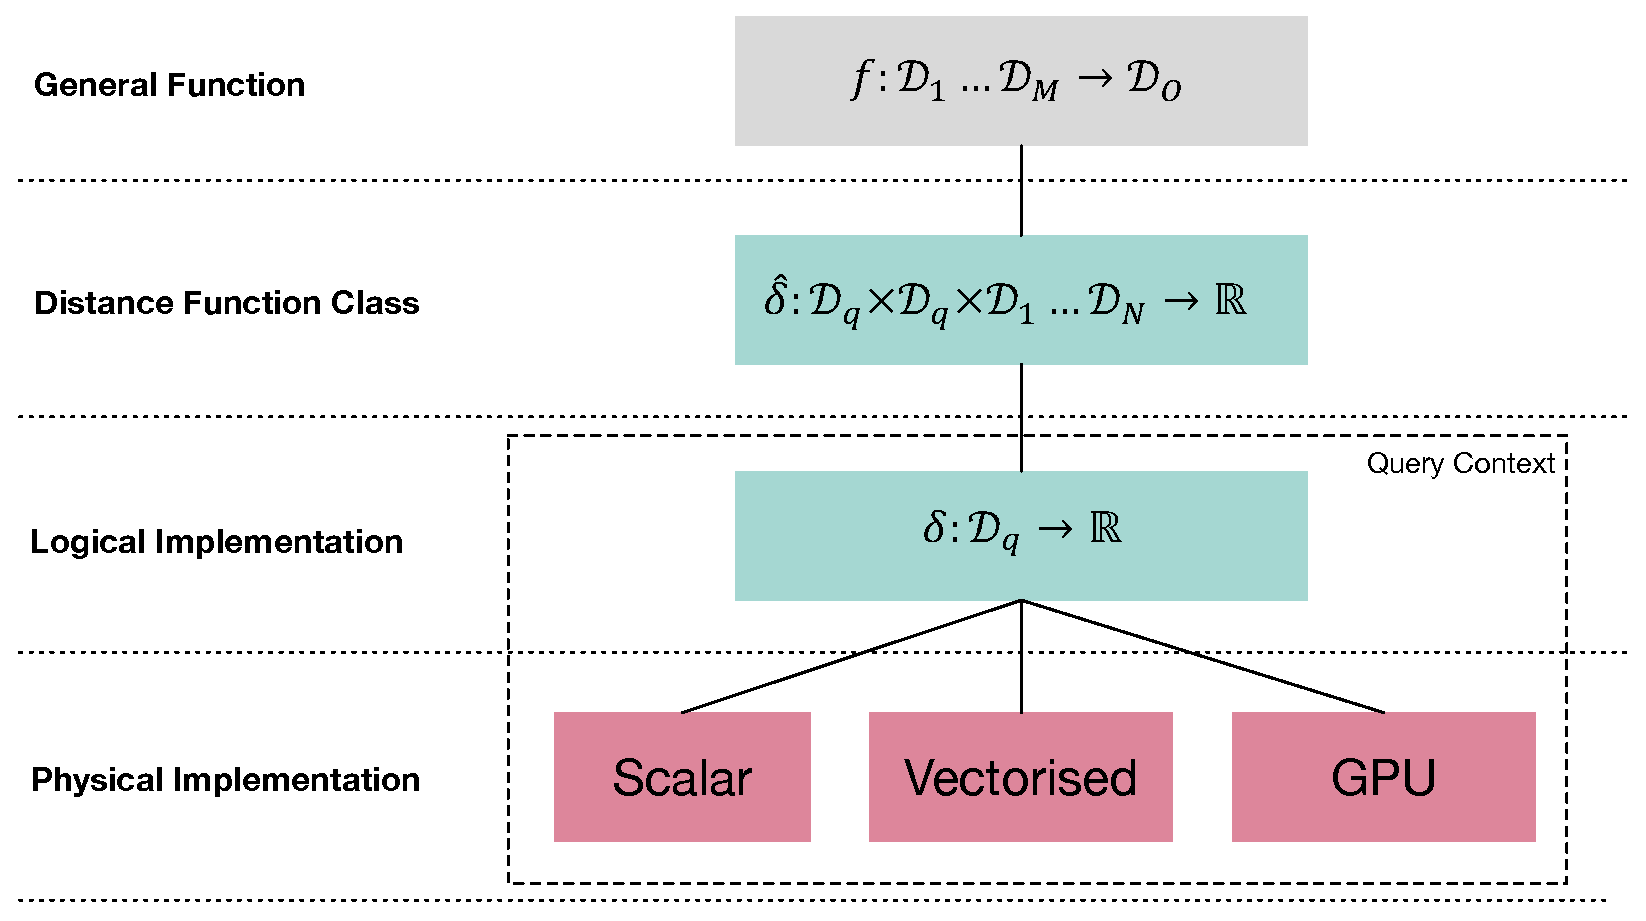
\includegraphics[width=\textwidth]{figures/function_hierarchy.eps}
    \caption{Function hierarchy of all $f \in \mathcal{F}$. As we go down the hierarchy, the \acrshort{dbms} gains knowledge about a function's structure.}
    \label{figure:function_hierarchy}
\end{figure}

\begin{description}
    \item[General Function] Every function $f \in \mathcal{F}$ is known with information about its name and domain (i.e., its signature $\mathtt{SIG}(f)$). This enables the \acrshort{dbms} to provide optimised implementations or replacements for composit operations.
    \item[Distance Function Class] Since DFCs constitute a specific type of function, we can embedd equivalences between a DFC and different types of index structures directly within the function registry. Those equivalences allow a query planner to select one over the other.
    \item[Logical Implementation] As an implementation of a query manifests, the structure of a DFC may change through implementation $\symdist = \mathtt{IMP}(\symdfc)$. For example, certain attributes may turn-out to remain constant, which can be leveraged by the planner to optimise execution.
    \item[Physical Implementation] As the physical execution plan emerges, a plan can make decisions as to what type of implementation for a DFC should be selected. For example, it may select a vectorised version, which leverages \acrshort{simd} instructions of the CPU, over a scalar implementation that calculates the distance in a tight loop.
\end{description}

\subsubsection{Functions and Optimised Implementations}

Optimising implementations of DFCs and general function invocations can be achieved in multiple ways. First, it is reasonable to provide and select implementations that are specific for the data type of the function arguments, so as to avoid type conversion in a tight loop over a large amount of data. From the perspective of execution performance, it is desirable to make this selection during planning rather than at query execution time.

Another aspect that can be optimised is the use of vectorized implementations for computations that involve vectors or matrices, i.e., exchanging a scalar implementation of a DFC by an implementation that uses \acrshort{simd} instructions. However, it is to expected that one challenge lies in finding the threshold after which usage of such an optimised version pays off. If we take real-valued vectors as an example, it is likely that vectorised execution will not benefit low-dimensional vectors (e.g., $dim = 3$) while it will greatly benefit high-dimensional vectors (e.g., $dim = 2048$). Finding this threshold poses challenge in and by itself, which could be subject for future research.

Finally, one can also try to match constellations of nested functions and replace them with optimised version. An example could be the expression $a * b + c$, i.e., $\mathtt{add}(\mathtt{mul}(a,b), c))$, which can be replaced by a single \emph{fused multiply-add} function $\mathtt{fma}(a,b,c)$ to avoid loss of precission. In a manner of speaking, trading-in a high-dimensional index for the execution of a DFC also falls into this category.

\subsubsection{DFCs and High-dimensional Index Structures}

One identity that is particularly relevant for the execution of proximity based queries is the relationship between the execution of a DFC and a high-dimensional index. While there are many different types of HD-indexes, we distinguish between three broader categories proposed by \cite{Lejsek:2018Transactional} and introduced and discussed in \Cref{chapter:theory_multimedia_analysis_and_retrieval}, namely \emph{quantization based} (e.g., \acrshort{pq} or \acrshort{vaf}), \emph{hash based} (e.g., \acrshort{lsh} or \acrshort{sh}) and \emph{tree based} (e.g., NV-tree \cite{Lejsek:2011NVTree}) indexes. We postulate the relationship between a high-dimensional index and a DFC given in \Cref{definition:dfc_and_index}. 

\begin{definition}[label=definition:dfc_and_index]{DFCs and high-dimensional index structures (exact case).}{}
    Let $\symdfc \colon \domain_q \times \domain_q \times \domain_{1} \ldots \times \domain_{n} \to \mathbb{R}$ be a \acrshort{dfc} and $\projection_{\mathcal{E}}$ be the extended projection involving execution of that DFC, i.e., $\symdfc \in \mathcal{E}$. A high-dimensional index $\mathtt{INDEX}$ is a pre-computed database object such that $\projection_{\symdfc(\cdot)}(\relation) = \mathtt{INDEX}(\relation)$ and therefore, the following equation holds:

    \begin{equation*}
        \projection_{\mathcal{E}} (\relation) = \projection_{\mathcal{E} \setminus \symdfc} (\relation) \Join \mathtt{INDEX} (\relation)
    \end{equation*}
    
    We call such an index \emph{exact} and we can use it as a replacement for the DFC.
\end{definition}

In addition to \Cref{definition:dfc_and_index}, the following restrictions apply (in addition to implementation specific restrictions for a specific index):

\begin{itemize}
    \item Indexes are always derived from a materialized relation $\relation$ and a feature attribute 
    $\attribute_f \in \schema(\relation)$. Therefore, an index can only replace a DFC if they operate on an unaltered version of $\attribute_f$. Changes to $\attribute_f$, e.g., through application of a nested function, will render the index unusable unless the same alteration was applied when creating the index.
    \item Indexes are usually trained for a specific distance function (e.g., Euclidean) or class of distance functions (e.g., Minkowski). Therefore, an index can only replace a DFC if that DFC coincides with the original function (-class).
\end{itemize}

With \Cref{definition:dfc_and_index} and the aforementioned, we have defined the basic relationship and rule that can be applied by a \acrshort{dbms}, when deciding whether or not to use a particular high-dimensional index structure. We will provide more insights into the nature of \emph{approximate} index structures in \Cref{section:cost_model}.

\pagebreak

\section{Cost Model for Retrieval Accuracy}
\label{section:cost_model}


As we have explained in \Cref{chapter:theory_databases}, most \acrshort{dbms} rely on a cost-model for planning and selecting the execution and access path of a user-specified query. In fact, ever since the System R paper \cite{Selinger:1979Access}, cost-based query planning and optimisation is considered a gold standard for database systems.

Must traditional \acrshort{dbms} exhibit comparatively simple cost-models that mainly rely on the cost incurred by accessing (reading / writing) pages from or to disk. Based on what has been discussed thus far, we argue that such a model has several shortcomings and that a cost model from multimedia databases should take the following aspects into account when chosing an execution path:

\begin{description}
    \item[Disk Access (IO)] Persistent storage and the access to information residing on disk is still the factor that contributes the most to long query execution times and is thus something, that a system should try to minimise \cite{Selinger:1979Access}.
    \item[CPU] Due to the computational complexity of proximity based operations, especially when high-dimensional vectors are involved, the processing time on CPU is a factor that can no longer be ignored and must thus be taken into account as well. For example, several index structures achieve speed-up by reducing the computational complexity of the operations involved \cite{Weber:1998Va,Jegou:2010Product}
    \item[Memory] Some algorithms, e.g., for sorting, can benefit greatly from pure in-memory processing as opposed to writing intermediate results to disk. While memory used to be a scarce resource, some environments allow for complete in-memory process even for very large datasets.
    \item[Inaccuracy] The inaccuracy of a result incurred, e.g., by the choice of a certain high-dimensional index structure \cite{Indyk1998:Approximate,Jegou:2010Product}, is a price that can be paid to attain speed-up but should be transparent to the system.
\end{description}

These factors can be used to characterise query workloads in a purely local setup consisting of a single node. For distributed databases, obviously, the cost incurred by data and message exchange must be considered as well. However, this is not in scope for the work presented in this Thesis. The aforementioned factors lead us to \Cref{definition:cost} for the cost incurred by a query execution plan $P$.

\begin{definition}[label=definition:cost]{Cost of a Query Exection Plan.}{}
    Let $P$ be an execution plan. The we call the 4-tuple $C = (c_{CPU}, c_{IO}, c_{MEM},c_{ACC})$ the \emph{cost} of $P$, which captures the atomic costs in terms of disk access (IO), CPU usage (CPU), memory usage (MEM) and accuracy (ACC).
\end{definition}

As we have argued in chapter \Cref{chapter:applications}, the requirements to a database system, especially in terms of robustness against inaccuracy is highly use-case dependent. Some use-cases can accept inaccuracy in the results while others cannot. Furthermore, there may be 

Describe cost model for execution plans with following properties:

\begin{itemize}
    \item Cost as a function of atomic costs: $f(a_{cpu}, a_{io}, a_{memory}, a_{accuracy}) \longrightarrow C$
    \item Means to estimate results accuracy and associated considerations from execution path (e.g., when using index) based on properties of the index
    \item Means to specify importance of accurate results (e.g., global, per-query, context-based i.e. when doing 1NN search) in comparison to other factors
    \item Systems perspective 1: How can such a cost model be applied during query planning and optimization?
\end{itemize}

\section{Adaptive Index Management}

\begin{figure}[h!]
    \centering
    \begin{subfigure}[b]{0.40\textwidth}
        \centering
        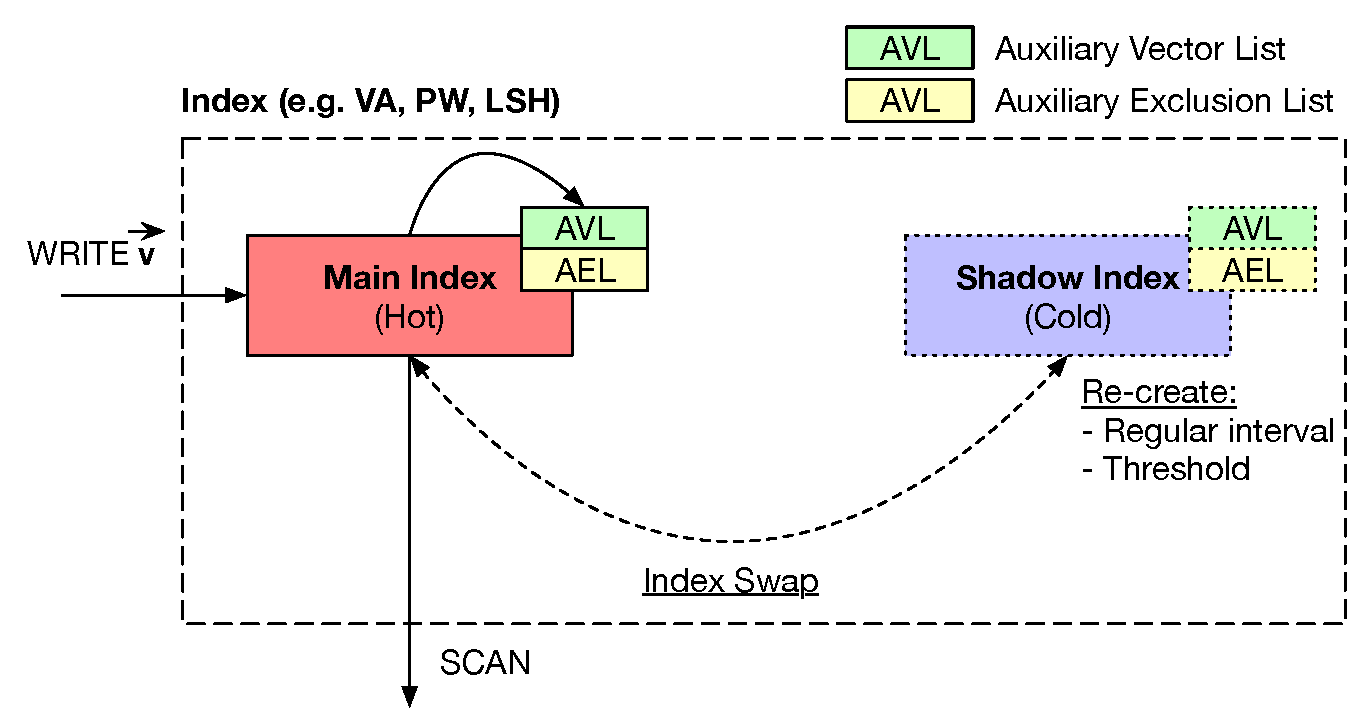
\includegraphics[width=\textwidth]{figures/adaptive_index.eps}
        \label{fig:adaptive_index:architecture}
    \end{subfigure}
    \hfill
    \begin{subfigure}[b]{0.40\textwidth}
        \centering
        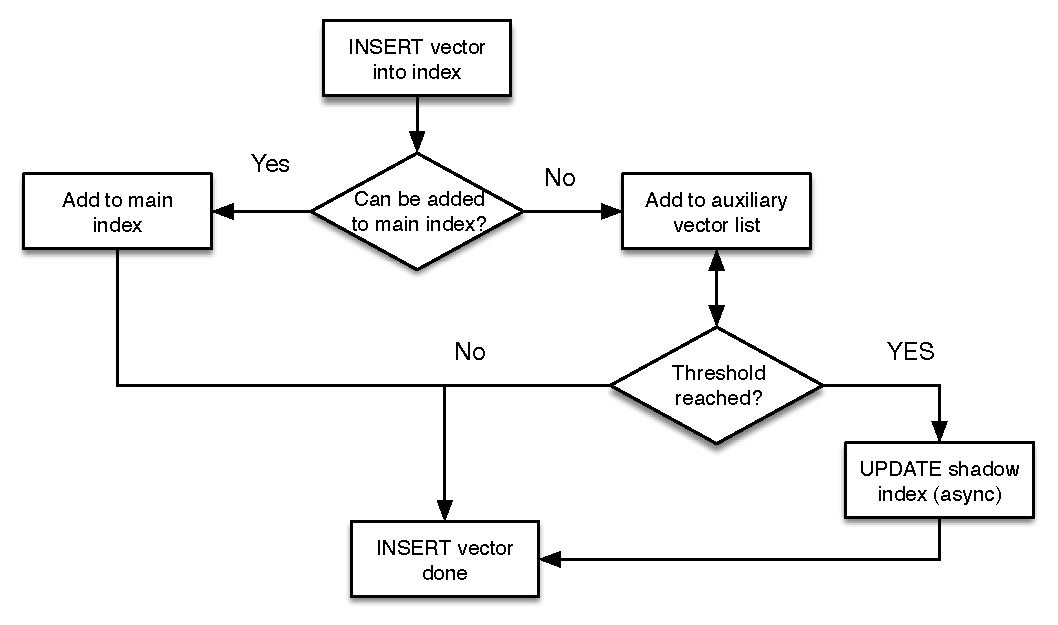
\includegraphics[width=\textwidth]{figures/adaptive_index_flow.eps}
        \label{fig:adaptive_index:flow}
    \end{subfigure}
    \caption{Adaptive index structures overview.}
    \label{fig:adaptive_index}
\end{figure}

Describe model for index management in the face of changing data (adaptive index management):

\begin{itemize}
    \item Reason about properties of secondary indexes for NNS (e.q., PQ, VA, LSH) with regards to data change
    \item Derivation of error bounds possible (e.g., usable for planning)?! Use in query planning?
    \item Systems perspective 1: How to cope with ``dirty'' indexes? Proposal: hot vs. cold index, auxilary data structure, offline optimization, see \cref{fig:adaptive_index}
    \item Systems perspective 2: On-demand index based on query workload?
\end{itemize}

\section{Architecture Model}

\todo[inline]{Putting everything together into a unified systems model (base on previous work + aforementioned aspects).}




